\chapter{Extension of the Supervision Architecture to Visiteuse 2}

\section*{Introduction}
\addcontentsline{toc}{section}{Introduction}
This chapter presents the extension of the stop-supervision system to \textit{Visiteuse 2}, a second production machine equipped with a Veichi VC3 PLC. The work focuses on adapting the PLC logic, Modbus TCP exchange, Node-RED processing, SQL insertion and HMI layers to this new machine.

\section{Positioning of the Extension}

\subsection{Extension Beyond the Initial Specifications}
The initial project focused on implementing a stop-supervision and stop-recording solution for one production machine. After this first implementation, the same functional principle was adapted to Visiteuse 2 in order to verify that it could be rebuilt on another PLC platform.

This extension represents an additional contribution to the project. It preserves the same operating principle: detection of a stop state, classification according to the stop duration, stop-cause selection, restart blocking for significant stops and database archiving.

The interest of this extension is both practical and technical. From a practical point of view, it gives the company a concrete example of how the supervision method can be reused. From a technical point of view, it required working with the Veichi VC3 PLC, the AutoStudio programming environment, the VI20 local HMI and a dedicated Node-RED communication profile.

\subsection{Technical Objectives}
The extension to Visiteuse 2 was structured around four objectives:

\begin{itemize}[leftmargin=1.1cm]
  \item develop a ladder program for the Veichi VC3 PLC while preserving the stop-recording principle used in the main project;
  \item configure Modbus TCP communication between Node-RED and the Veichi PLC according to the VC3 addressing convention;
  \item integrate the stop data into the existing SQL recording logic used by the project;
  \item provide two complementary interfaces: a VI20 local HMI near the machine and a browser-based web HMI for centralized supervision.
\end{itemize}

\begin{figure}[H]
\centering
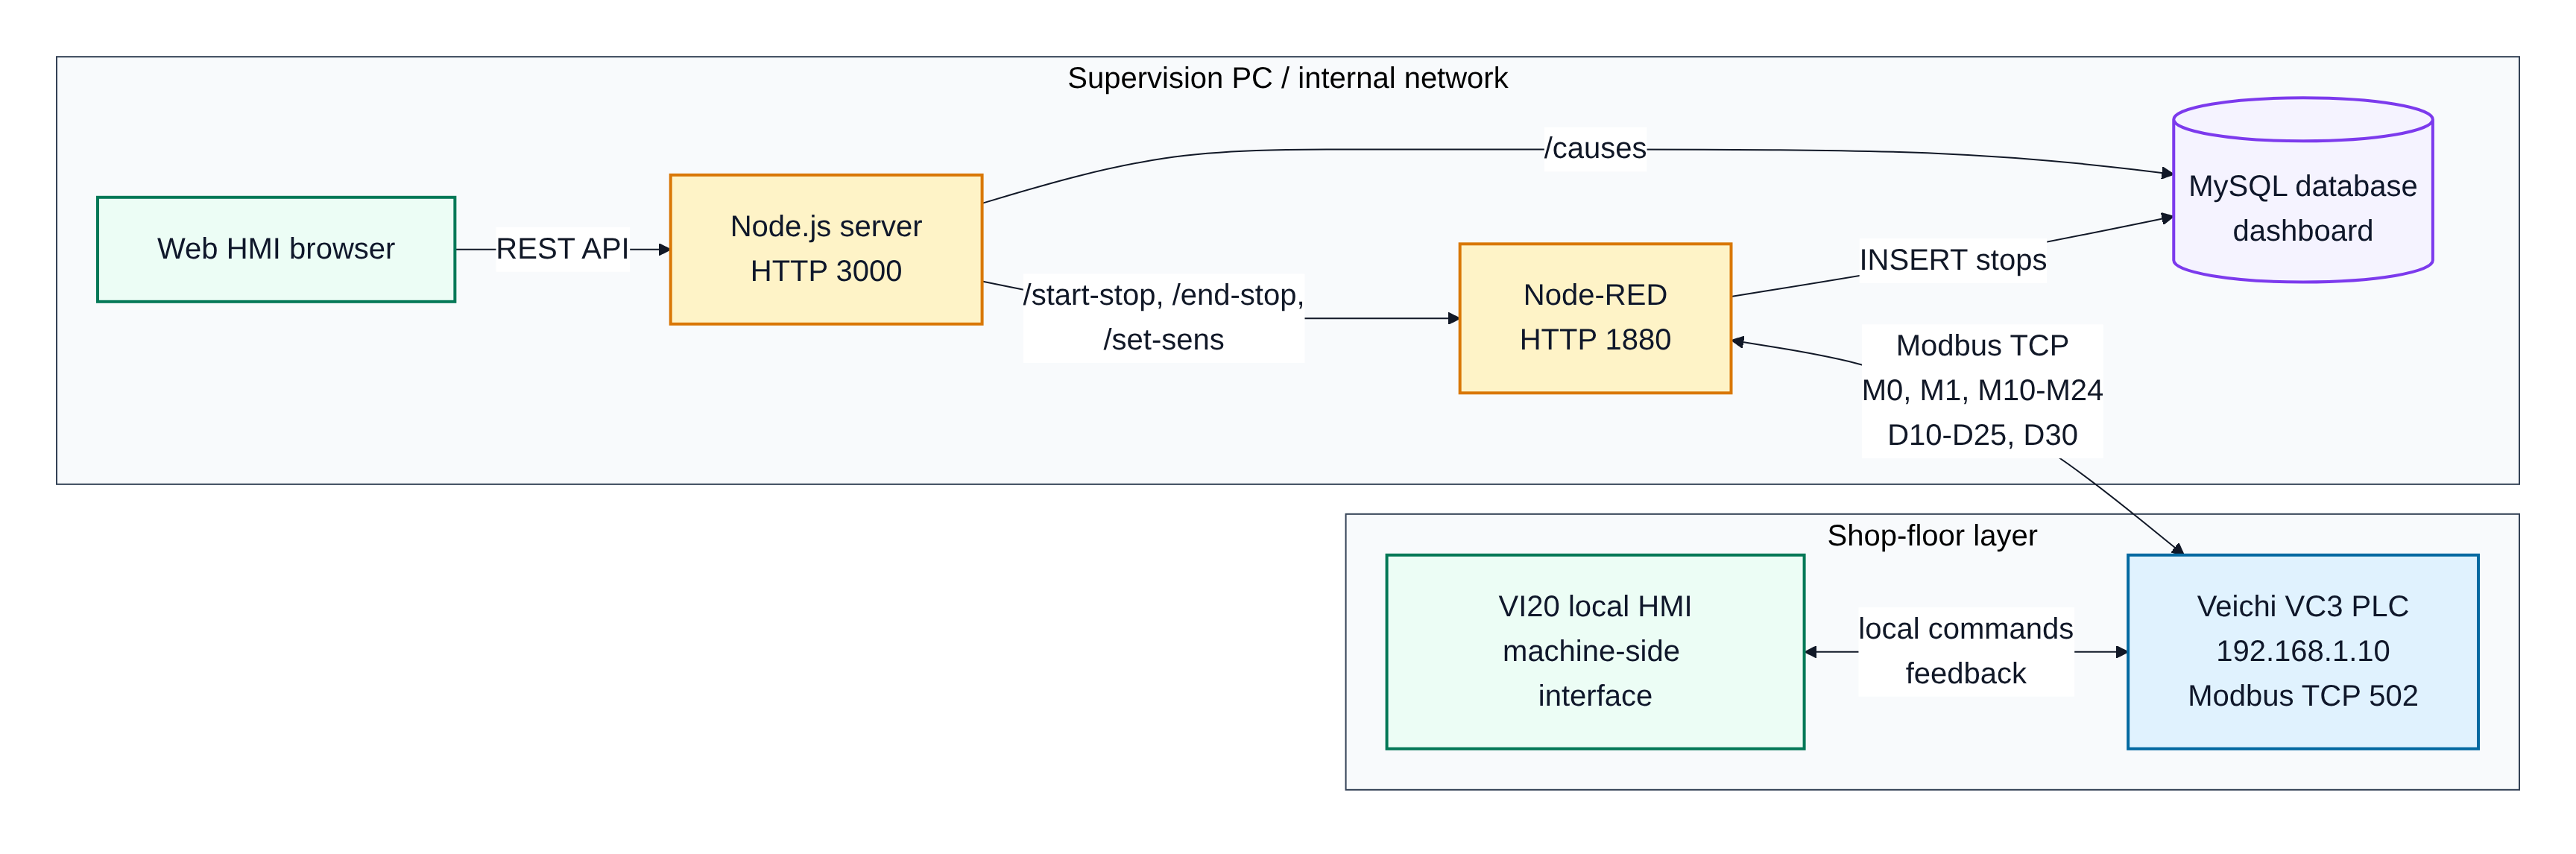
\includegraphics[width=0.9\textwidth, keepaspectratio]{images/fig_01_deployment_visiteuse2.png}
\caption{Deployment Architecture of the Supervision Extension Applied to Visiteuse 2}
\label{fig:chapter4-1}
\end{figure}

\section{Implementation Methodology}

\subsection{Adopted Work Methodology}
The implementation followed a layered sequence. The PLC layer was developed first because it contains the stop-cycle logic and the timestamp preparation. The communication layer was then configured in Node-RED to exchange data with the PLC. Finally, the local HMI and the web HMI were connected to the same functional logic.

The adopted development order was as follows:

\begin{enumerate}[leftmargin=1.2cm]
  \item programming the ladder logic of Visiteuse 2 in AutoStudio;
  \item configuring Modbus TCP communication for the Veichi VC3 address map;
  \item decoding the stop data and preparing the SQL insertion path;
  \item developing the web HMI and its API calls through the Node.js server;
  \item designing the local HMI on the Veichi screen using VI20;
  \item validating the short-stop and long-stop scenarios through the HMI and SQL records.
\end{enumerate}

Each layer has a defined role. The PLC handles real-time stop logic, Node-RED manages Modbus exchange and SQL insertion, the Node.js server exposes the web interface and REST API, MySQL stores the stop records, and the HMI screens provide operator interaction.

\begin{table}[H]
\centering
\caption{Responsibilities of the main components used for Visiteuse 2}
\resizebox{\textwidth}{!}{%
\begin{tabular}{|l|p{10cm}|}
\hline
\textbf{Component} & \textbf{Responsibility} \\
\hline
Veichi VC3 PLC & Detects the stop cycle, applies the 30-second rule, manages restart blocking and prepares timestamp/cause data. \\
\hline
VI20 local HMI & Provides the shop-floor operator interface near the machine. \\
\hline
Node-RED & Reads and writes Modbus TCP variables, retrieves stop data and inserts stop records into MySQL. \\
\hline
Node.js server & Serves the web HMI, exposes REST endpoints and forwards web commands to Node-RED. \\
\hline
MySQL database & Stores stop records and cause labels used by the supervision system. \\
\hline
Web HMI & Provides centralized supervision and non-safety operator interaction from the internal network. \\
\hline
\end{tabular}%
}
\end{table}

\subsection{Preserved Functional Principle}
The functional rule used for Visiteuse 2 is based on the same distinction between micro-stops and significant stops:

\begin{itemize}[leftmargin=1.1cm]
  \item a stop lasting less than 30 seconds is automatically classified with cause \texttt{16};
  \item a stop lasting 30 seconds or more requires the operator to select a valid cause from causes \texttt{1-15} before the stop cycle is closed.
\end{itemize}

This rule avoids unnecessary manual recording of very short stops while keeping traceability for significant production losses.

\begin{figure}[H]
\centering
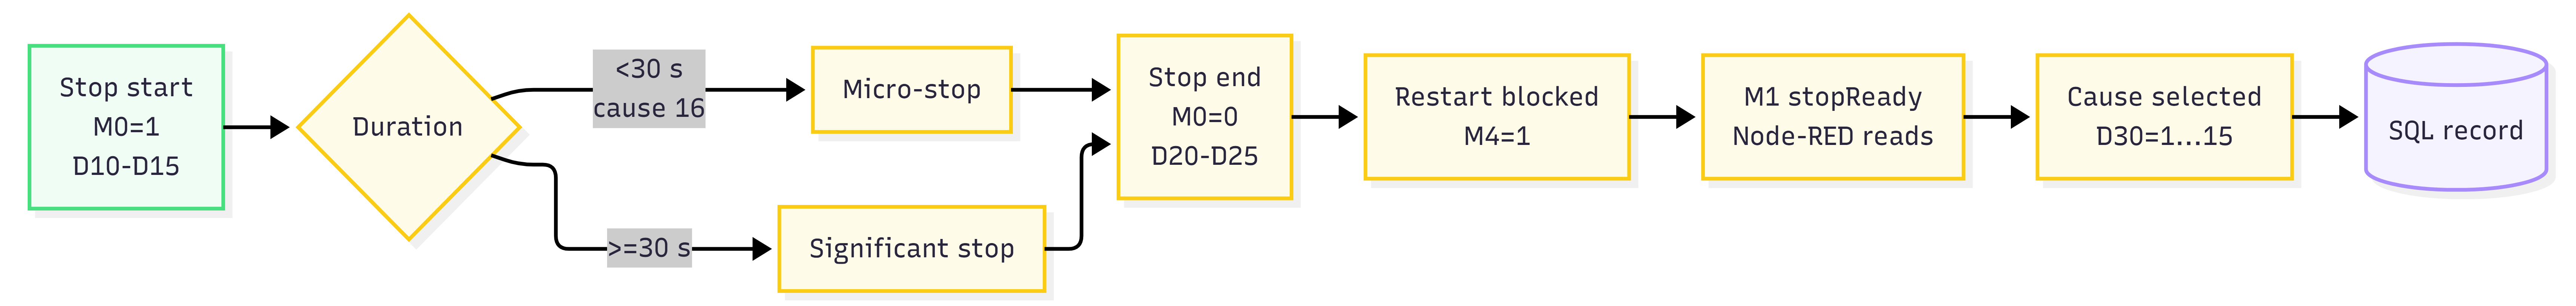
\includegraphics[width=0.9\textwidth, keepaspectratio]{images/fig_02_stop_scenario_visiteuse2.png}
\caption{Functional Stop Scenario on Visiteuse 2}
\label{fig:chapter4-2}
\end{figure}

\section{Programming and Control Logic}

\subsection{Ladder Development in AutoStudio}
For Visiteuse 2, a new ladder program was developed in AutoStudio for the Veichi VC3 PLC. The program was not copied directly from the first machine; it was rebuilt according to the Veichi environment, its variables, its instructions and its timer behavior.

The ladder logic is organized around the following functions:

\begin{itemize}[leftmargin=1.1cm]
  \item using \texttt{isStopped} at address \texttt{M0} as the stop-state/control bit of the implemented supervision logic;
  \item recording the stop-start timestamp in \texttt{D10-D15};
  \item resetting \texttt{D30}, \texttt{stopReady}, \texttt{causeSelected}, \texttt{restartBlocked} and cause bits at the beginning of a stop cycle;
  \item applying a 30-second timer to identify significant stops;
  \item blocking restart when a significant stop has no selected cause;
  \item converting cause bits \texttt{M10-M24} into the numeric cause identifier stored in \texttt{D30};
  \item recording the stop-end timestamp in \texttt{D20-D25};
  \item setting \texttt{stopReady} at \texttt{M1} so that Node-RED can read the prepared stop data.
\end{itemize}

In the current implementation, \texttt{M0} is named \texttt{isStopped} in the PLC variable table and is also written by the web command path through Node-RED. It is therefore described as an internal stop-state/control bit used by the supervision logic.

\begin{figure}[H]
\centering
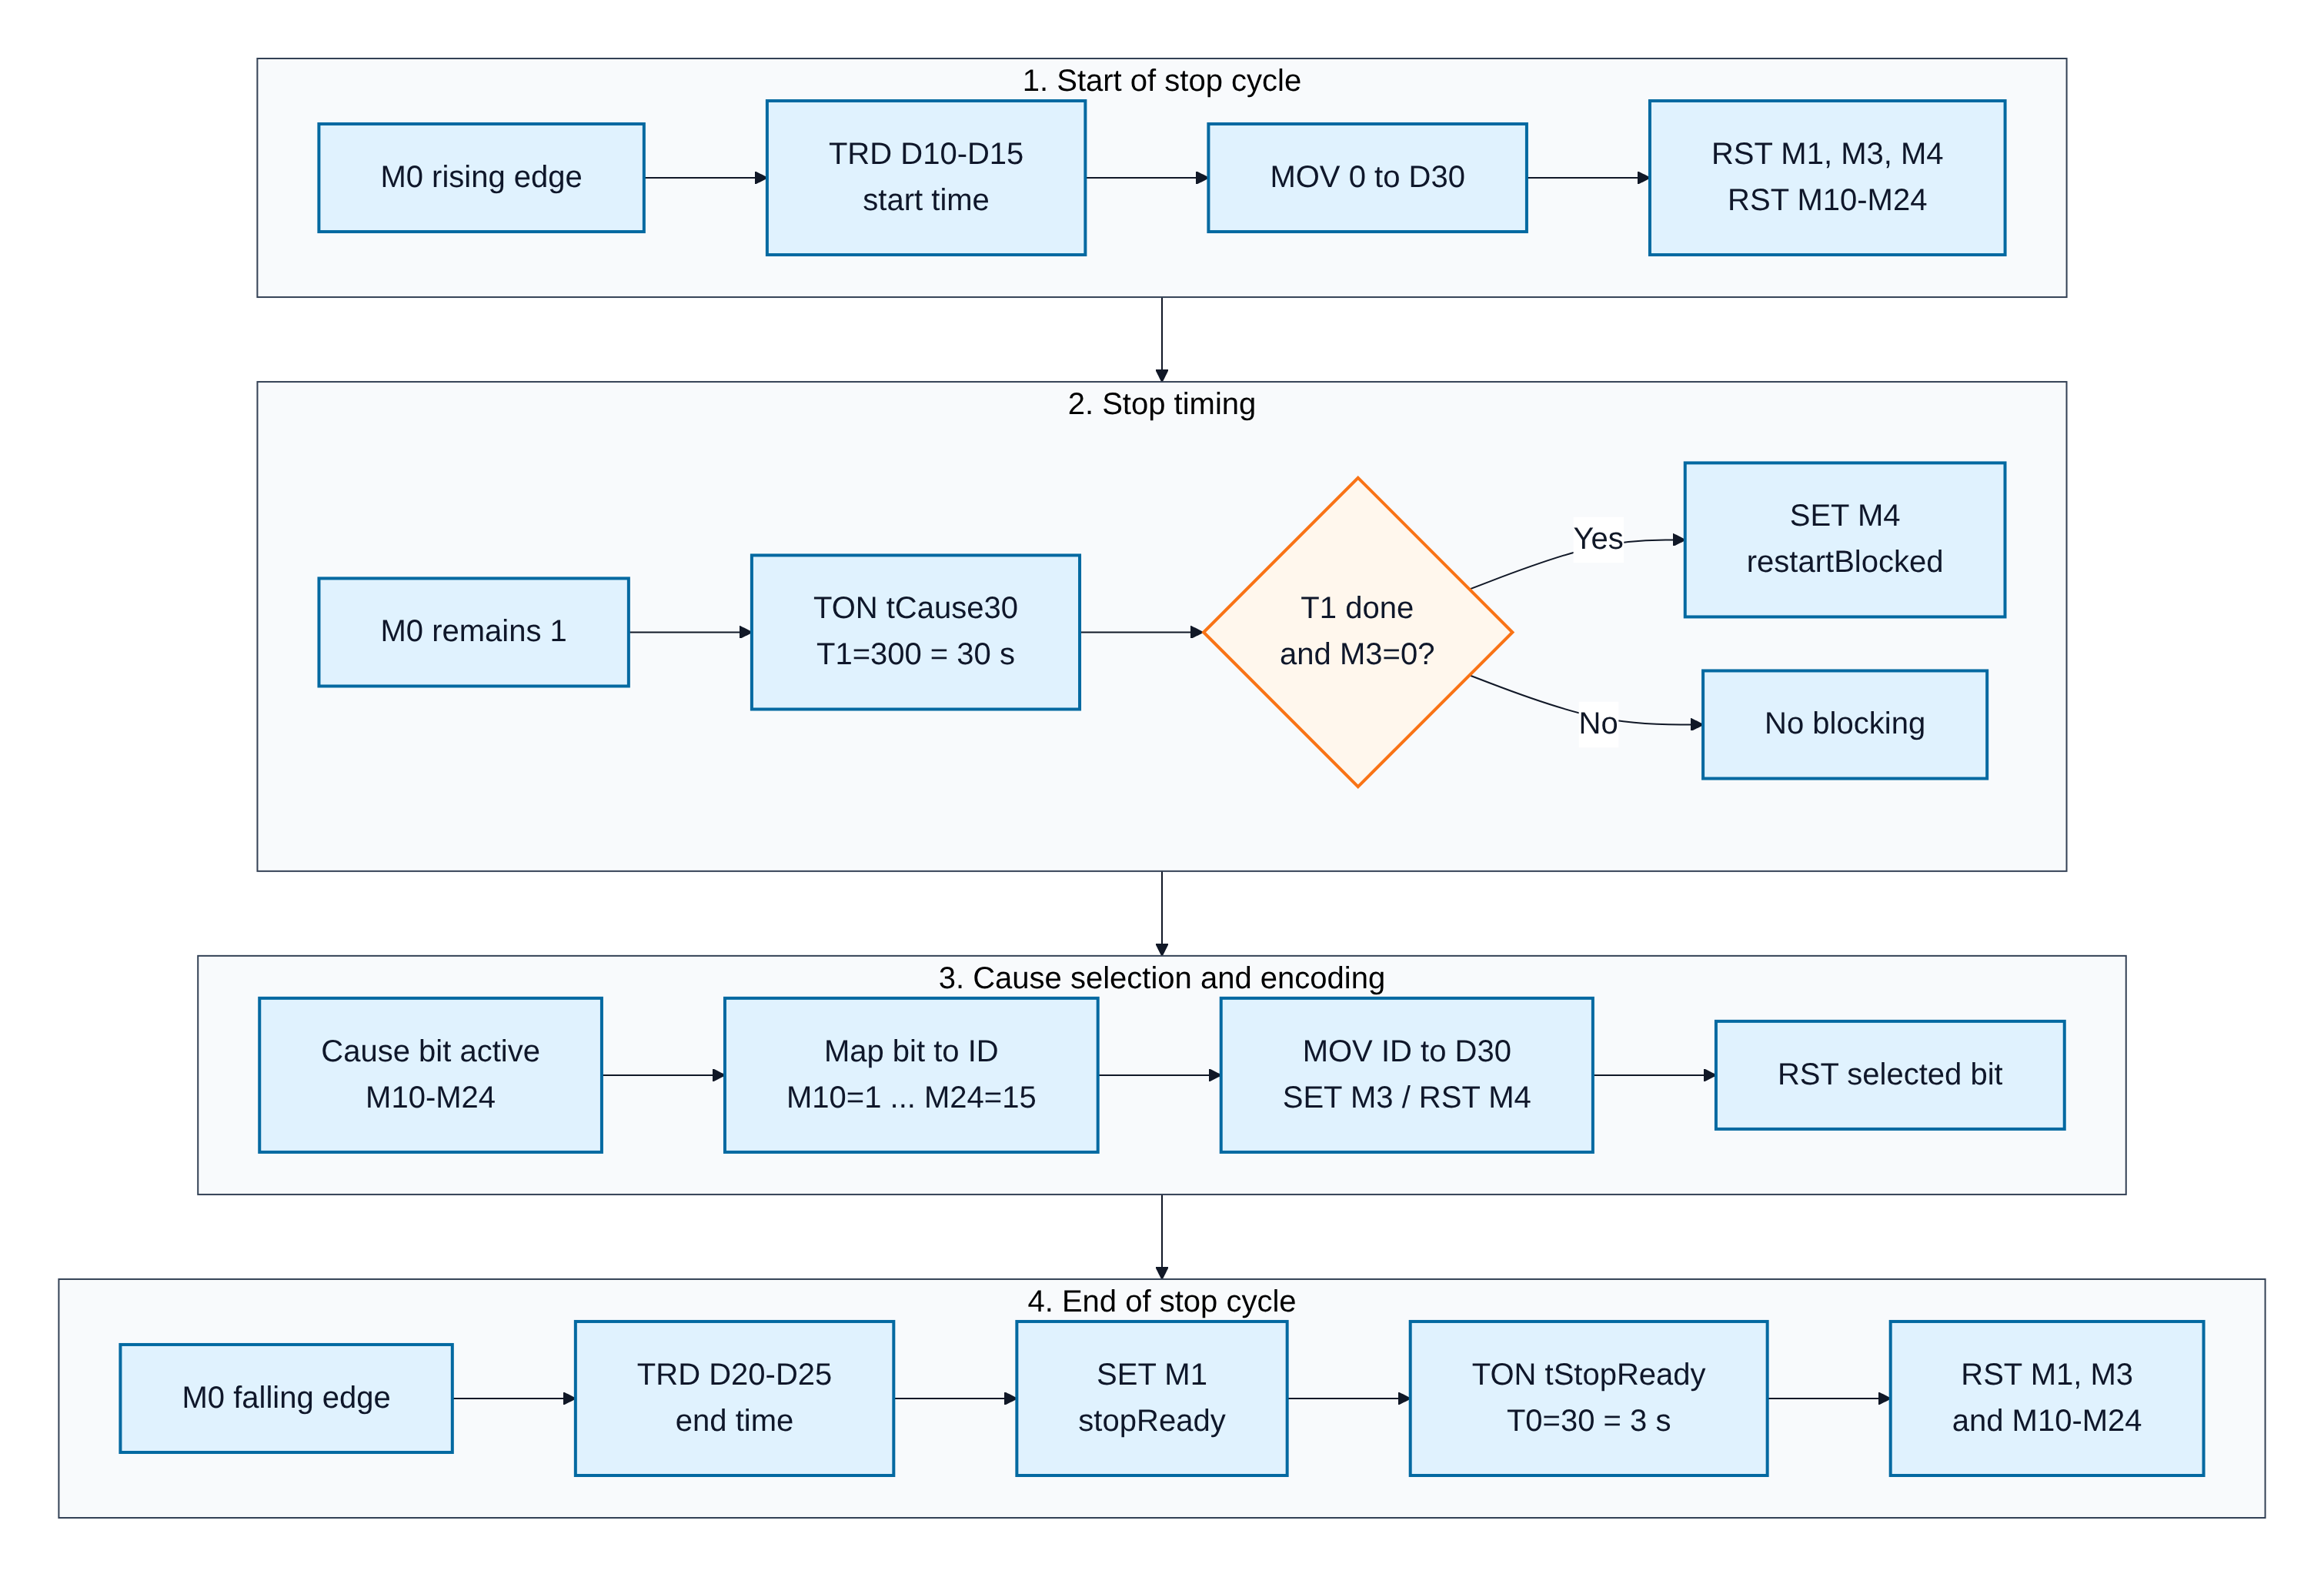
\includegraphics[width=0.9\textwidth, keepaspectratio]{images/fig_03_autostudio_ladder_structure.png}
\caption{Logical Structure of the Ladder Program Developed in AutoStudio}
\label{fig:chapter4-3}
\end{figure}

\subsection{Timer Adaptation Through TON Blocks}
Only two timers are essential in this extension. The first timer, \texttt{tCause30}, detects whether the stop has reached the 30-second threshold. The second timer, \texttt{tStopReady}, keeps \texttt{M1/stopReady} active for a short period after the stop data have been prepared.

\begin{table}[H]
\centering
\caption{Timer and synchronization parameters used in the implementation}
\resizebox{\textwidth}{!}{%
\begin{tabular}{|l|l|p{6cm}|}
\hline
\textbf{Parameter} & \textbf{Value} & \textbf{Function} \\
\hline
\texttt{tCause30} & \texttt{T1 = 300 = 30 s} & Threshold used to distinguish micro-stops from significant stops. \\
\hline
\texttt{tStopReady} & \texttt{T0 = 30 = 3 s} & Holds \texttt{M1/stopReady} long enough for Node-RED to detect the event. \\
\hline
Node-RED polling period & \texttt{500 ms} & Polling period used to read \texttt{M1}. \\
\hline
Stabilization delay & \texttt{100 ms} & Delay applied before extracting the timestamp and cause registers after \texttt{M1} becomes active. \\
\hline
Cause-to-restart delay & \texttt{200 ms} & Delay applied after writing the selected cause bit and before resetting \texttt{M0}. \\
\hline
\end{tabular}%
}
\end{table}

\subsection{PLC Synchronization and Variables Used}
The synchronization between PLC control, HMI interaction and Node-RED communication is based on a limited set of bits, timers and registers.

\begin{table}[H]
\centering
\caption{Main variables used in the Visiteuse 2 ladder program}
\resizebox{\textwidth}{!}{%
\begin{tabular}{|l|l|p{6.5cm}|}
\hline
\textbf{Variable} & \textbf{PLC address} & \textbf{Functional role} \\
\hline
\texttt{isStopped} & \texttt{M0} & Internal stop-state/control bit. It is set to \texttt{1} when the stop cycle starts and reset to \texttt{0} when the stop cycle is closed. \\
\hline
\texttt{stopReady} & \texttt{M1} & Indicates that the stop data are ready for Node-RED reading. \\
\hline
\texttt{tStopReady} & \texttt{T0} & Keeps \texttt{stopReady} active for approximately 3 seconds. \\
\hline
\texttt{causeSelected} & \texttt{M3} & Confirms that a cause has been selected during a significant stop. \\
\hline
\texttt{restartBlocked} & \texttt{M4} & Blocks restart authorization when the stop reaches 30 seconds and no valid cause has been selected. \\
\hline
\texttt{tCause30} & \texttt{T1} & 30-second timer used to classify a stop as significant. \\
\hline
\texttt{M10-M24} & Cause bits & Bits used to transmit causes \texttt{1-15} to the PLC. \\
\hline
\texttt{D10-D15} & D registers & Stop-start timestamp generated by the \texttt{TRD} instruction. \\
\hline
\texttt{D20-D25} & D registers & Stop-end timestamp generated by the \texttt{TRD} instruction. \\
\hline
\texttt{D30} & D register & Numeric identifier of the selected cause for significant stops. For micro-stops, Node-RED archives cause \texttt{16}. \\
\hline
\end{tabular}%
}
\end{table}

\subsection{Timestamp Register Format}
The \texttt{TRD} instruction stores timestamp fields in the order year, month, day, hour, minute and second. Node-RED reconstructs the start and end times from these registers before inserting the stop record.

\begin{table}[H]
\centering
\caption{Timestamp register format used by Node-RED}
\resizebox{\textwidth}{!}{%
\begin{tabular}{|l|l|p{6cm}|}
\hline
\textbf{Register} & \textbf{Field} & \textbf{Format used} \\
\hline
\texttt{D10} / \texttt{D20} & Year & Numeric value. Two-digit values are normalized as \texttt{2000 + value}. \\
\hline
\texttt{D11} / \texttt{D21} & Month & Numeric value from \texttt{1} to \texttt{12}. \\
\hline
\texttt{D12} / \texttt{D22} & Day & Numeric value from \texttt{1} to \texttt{31}. \\
\hline
\texttt{D13} / \texttt{D23} & Hour & Numeric value from \texttt{0} to \texttt{23}. \\
\hline
\texttt{D14} / \texttt{D24} & Minute & Numeric value from \texttt{0} to \texttt{59}. \\
\hline
\texttt{D15} / \texttt{D25} & Second & Numeric value from \texttt{0} to \texttt{59}. \\
\hline
\end{tabular}%
}
\end{table}

\subsection{Stop-Cause Encoding}
The stop causes selected by the operator are transmitted as bits. Each bit corresponds to one cause identifier. The ladder program converts the active bit into the numeric value stored in \texttt{D30}.

\begin{table}[H]
\centering
\caption{Correspondence between cause bits and the value stored in \texttt{D30}}
\resizebox{\textwidth}{!}{%
\begin{tabular}{|c|c|c|c|c|c|}
\hline
\textbf{Bit} & \textbf{Cause ID} & \textbf{Bit} & \textbf{Cause ID} & \textbf{Bit} & \textbf{Cause ID} \\
\hline
\texttt{M10} & 1 & \texttt{M15} & 6 & \texttt{M20} & 11 \\
\hline
\texttt{M11} & 2 & \texttt{M16} & 7 & \texttt{M21} & 12 \\
\hline
\texttt{M12} & 3 & \texttt{M17} & 8 & \texttt{M22} & 13 \\
\hline
\texttt{M13} & 4 & \texttt{M18} & 9 & \texttt{M23} & 14 \\
\hline
\texttt{M14} & 5 & \texttt{M19} & 10 & \texttt{M24} & 15 \\
\hline
\end{tabular}%
}
\end{table}

Cause \texttt{16} is reserved for automatically classified micro-stops. It is not transmitted to the PLC as a manual cause bit.

\section{Industrial Connectivity and SQL Integration}

\subsection{Node-RED Configuration for the Veichi Profile}
After the ladder program was implemented, the Node-RED layer was adapted to communicate with the Veichi VC3 PLC. This step required a dedicated communication profile for the IP address, the Modbus TCP port, the unit identifier and the VC3 address mapping.

\begin{table}[H]
\centering
\caption{Main communication parameters for the Veichi VC3 PLC}
\resizebox{\textwidth}{!}{%
\begin{tabular}{|l|p{8cm}|}
\hline
\textbf{Parameter} & \textbf{Value used} \\
\hline
PLC & Veichi VC3 \\
\hline
PLC programming software & AutoStudio \\
\hline
PLC IP address & \texttt{192.168.1.10} \\
\hline
Protocol & Modbus TCP \\
\hline
Port & \texttt{502} \\
\hline
Unit ID & \texttt{1} \\
\hline
Modbus client name in Node-RED & \texttt{veichi-vc3-m-2000} \\
\hline
Modbus address of \texttt{M0} & Coil/protocol address \texttt{2000} \\
\hline
Modbus address of \texttt{M1} & Coil/protocol address \texttt{2001} \\
\hline
Modbus addresses of \texttt{M10-M24} & Coil/protocol addresses \texttt{2010-2024} \\
\hline
Timestamp and cause registers & Holding-register block starting at address \texttt{10}, with useful fields \texttt{D10-D15}, \texttt{D20-D25} and \texttt{D30}. \\
\hline
\end{tabular}%
}
\end{table}

The main addressing difference concerns the \texttt{M} bits. In AutoStudio the variables are named \texttt{M0}, \texttt{M1}, \texttt{M10} and so on, whereas the Node-RED Modbus profile accesses them through Veichi protocol addresses: \texttt{M0 = 2000}, \texttt{M1 = 2001} and \texttt{M10-M24 = 2010-2024}.

\subsection{Reading Stop Data}
Node-RED periodically reads \texttt{M1/stopReady}. When this bit becomes active, the flow detects the rising edge, waits 100 ms and extracts the useful stop fields: \texttt{D10-D15} for the start timestamp, \texttt{D20-D25} for the end timestamp and \texttt{D30} for the selected cause.

\begin{table}[H]
\centering
\caption{Useful registers extracted by Node-RED}
\resizebox{\textwidth}{!}{%
\begin{tabular}{|l|l|p{6cm}|}
\hline
\textbf{Registers} & \textbf{Data} & \textbf{Description} \\
\hline
\texttt{D10-D15} & Stop start & Year, month, day, hour, minute and second of the stop start. \\
\hline
\texttt{D20-D25} & Stop end & Year, month, day, hour, minute and second of the stop end. \\
\hline
\texttt{D30} & PLC cause & Operator cause identifier for significant stops. \\
\hline
\end{tabular}%
}
\end{table}

If the calculated duration is less than 30 seconds, Node-RED archives cause \texttt{16}. If the duration is greater than or equal to 30 seconds, Node-RED uses the value read from \texttt{D30}, provided that it is between \texttt{1} and \texttt{15}.

\begin{figure}[H]
\centering
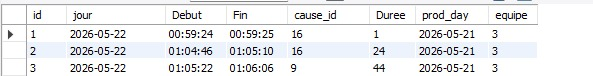
\includegraphics[width=0.9\textwidth, keepaspectratio]{images/sql_stop_records_example.jpeg}
\caption{Example of Stop Records Inserted into the SQL Database}
\label{fig:chapter4-4}
\end{figure}

\begin{figure}[H]
\centering
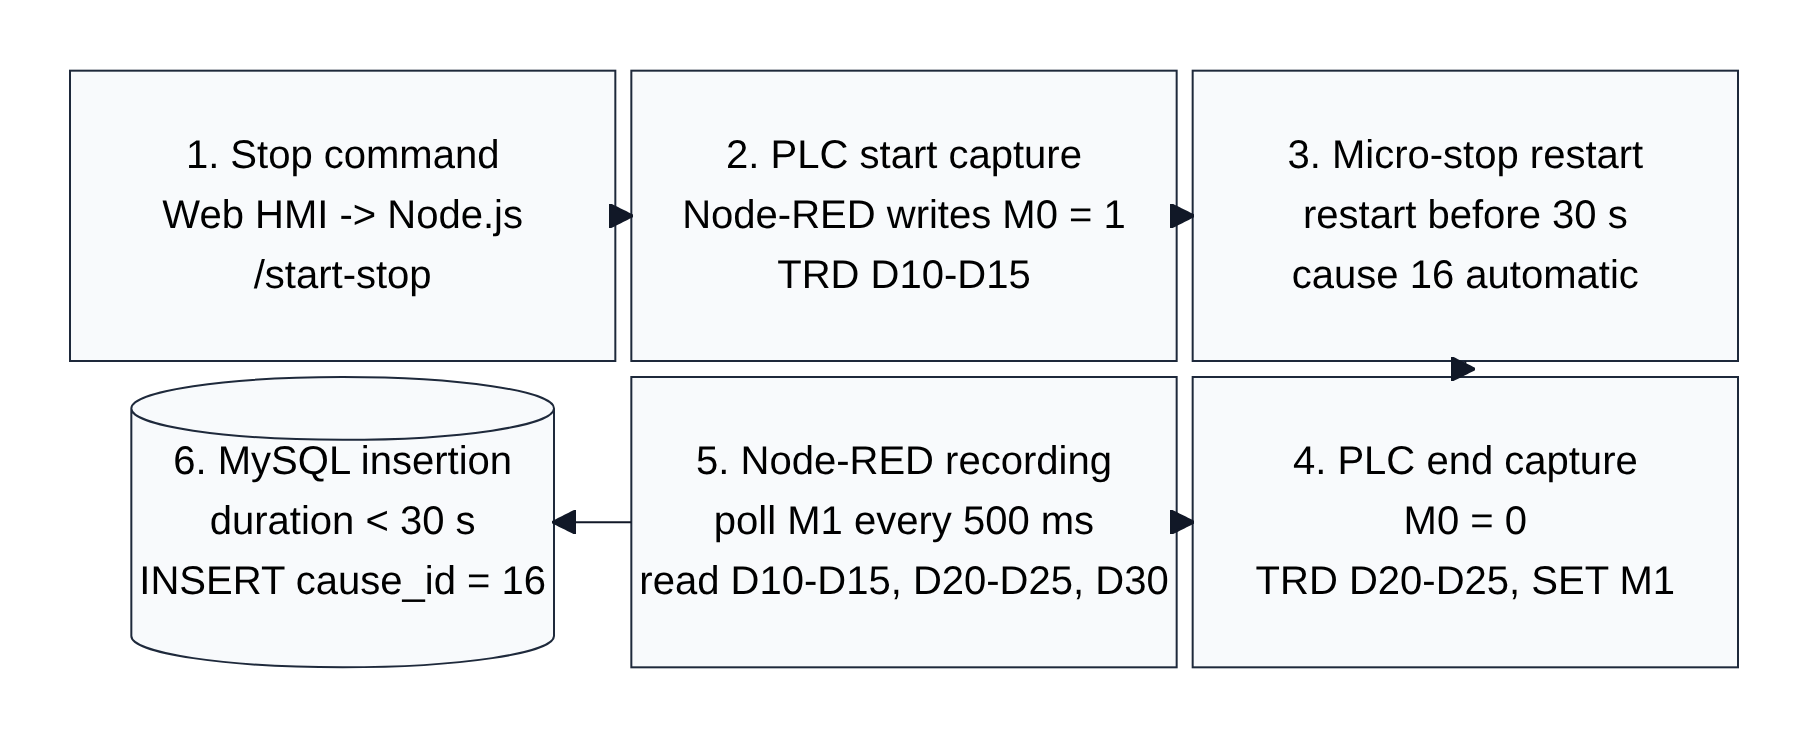
\includegraphics[width=0.9\textwidth, keepaspectratio]{images/fig_04_short_stop_sequence_visiteuse2.png}
\caption{Short-Stop Communication Sequence Used for Automatic Micro-Stop Recording}
\label{fig:chapter4-5}
\end{figure}

\begin{figure}[H]
\centering
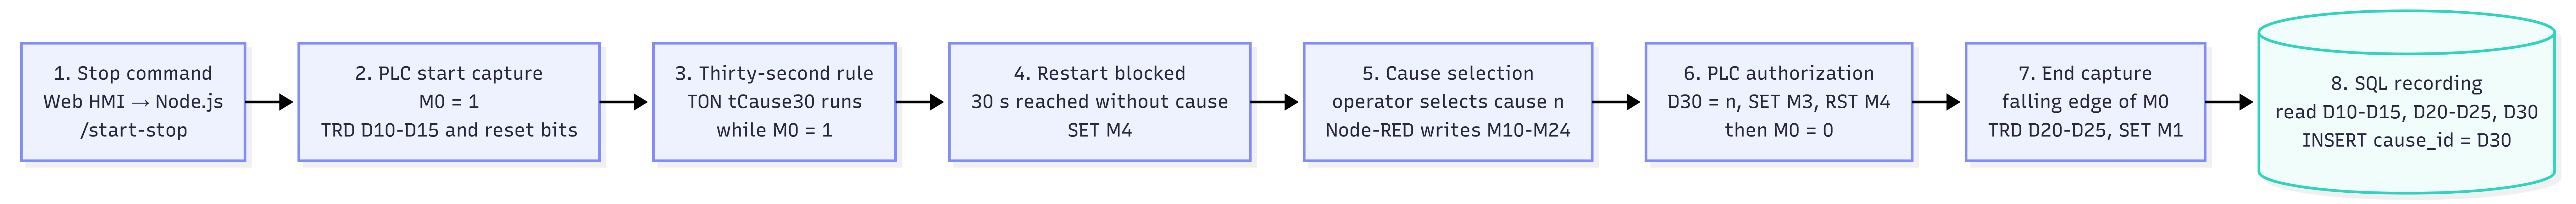
\includegraphics[width=0.9\textwidth, keepaspectratio]{images/fig_05_long_stop_sequence_visiteuse2.png}
\caption{Long-Stop Communication Sequence with Mandatory Cause Selection}
\label{fig:chapter4-6}
\end{figure}

\begin{figure}[H]
\centering
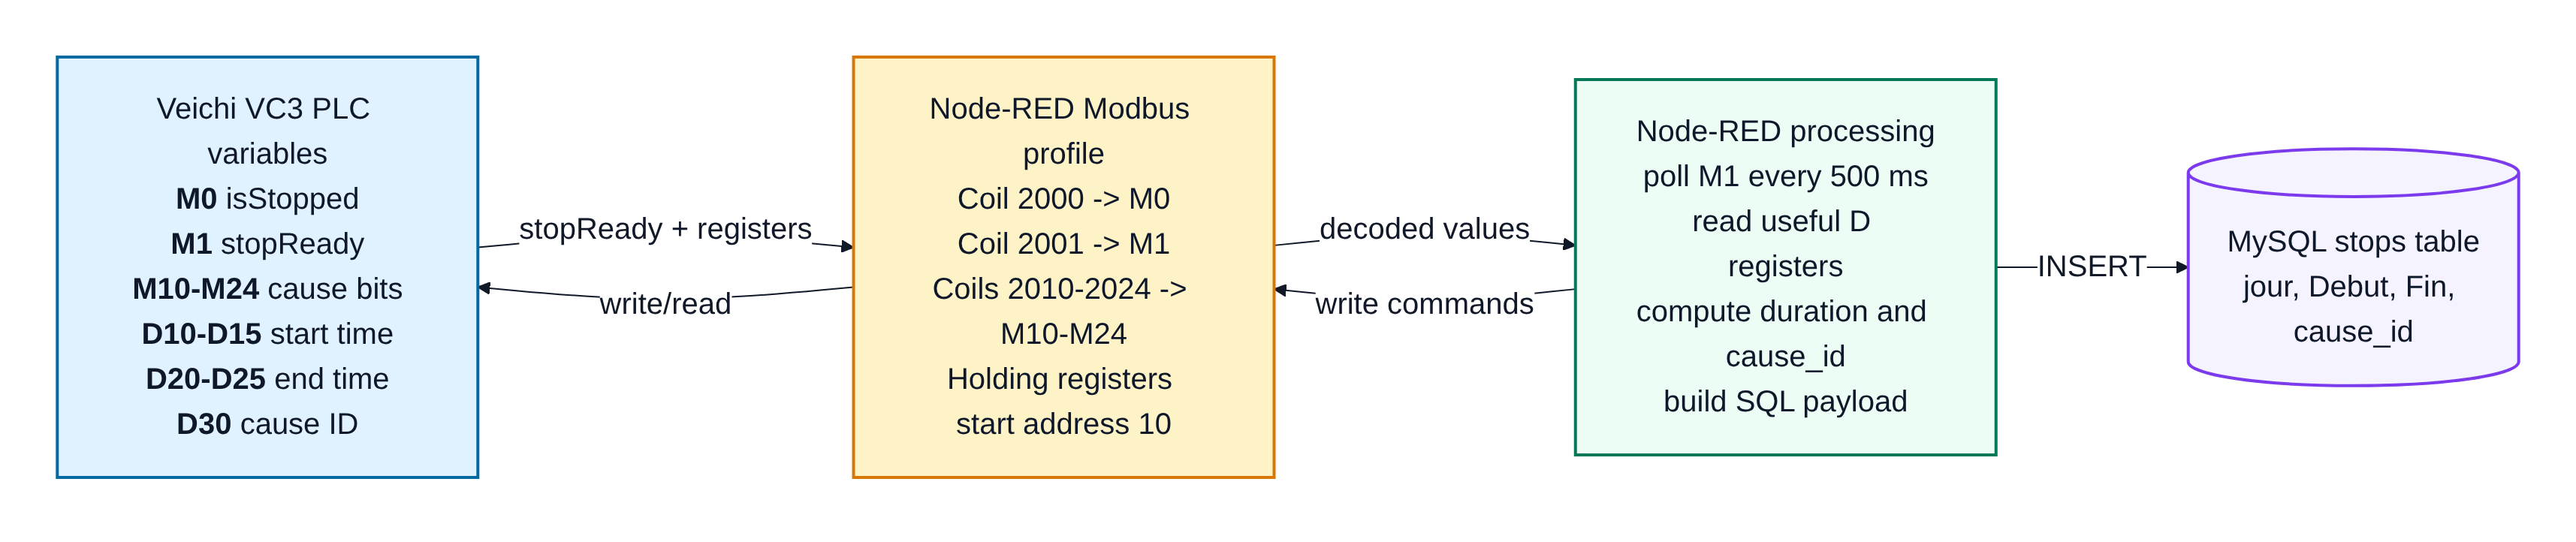
\includegraphics[width=0.9\textwidth, keepaspectratio]{images/fig_06_modbus_mapping_veichi.png}
\caption{Mapping of Visiteuse 2 Variables in Modbus TCP Communication}
\label{fig:chapter4-7}
\end{figure}

\subsection{Integration with the Existing SQL Recording Logic}
The SQL database had already been implemented during the main project. For this extension, Node-RED reuses the existing stop-recording path and inserts the fields \texttt{jour}, \texttt{Debut}, \texttt{Fin} and \texttt{cause\_id}. The remaining analysis fields, such as duration, production day and team, are computed by the existing SQL logic.

The web HMI also retrieves active cause labels from the database through the \texttt{/causes} endpoint. Cause \texttt{16} is excluded from manual selection because it is reserved for automatic micro-stop classification.

\section{Development of Supervision Interfaces}

\subsection{Local Veichi HMI Developed with VI20}
A local HMI was developed on the Veichi touch screen using VI20. This interface is intended for the operator positioned near the machine. It provides local supervision of Visiteuse 2 and direct access to the main operating commands.

Within this extension, the local HMI is complemented by the web HMI. The two interfaces are not alternatives: the local HMI remains the field interface, while the web HMI provides centralized access from the internal network.

\begin{figure}[H]
\centering
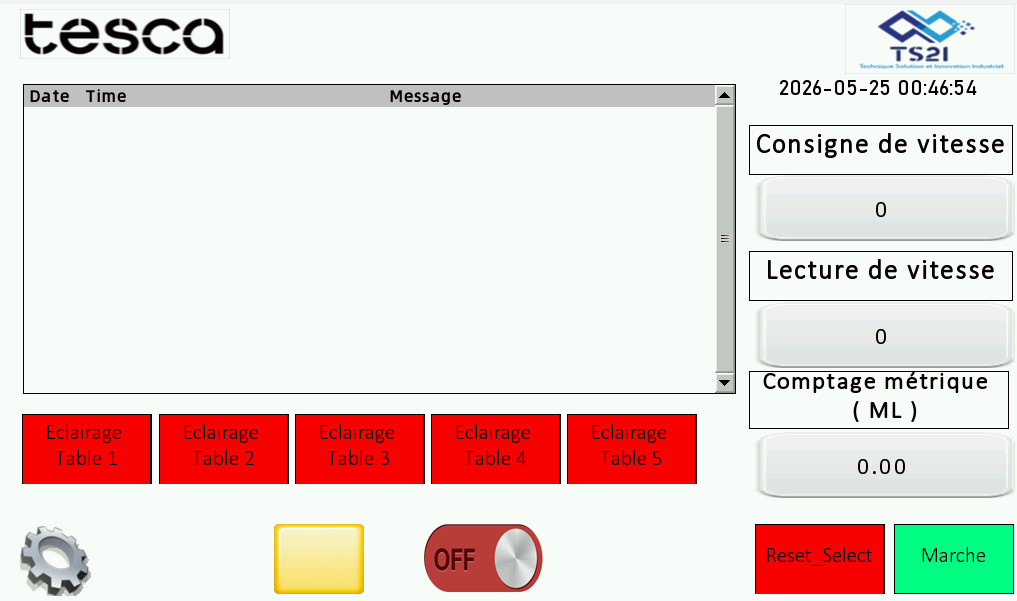
\includegraphics[width=0.75\textwidth, keepaspectratio]{images/hmi_veichi_vi20_main_screen.png}
\caption{Veichi VI20 Local HMI - Main Operating Screen}
\label{fig:chapter4-8}
\end{figure}

\begin{figure}[H]
\centering
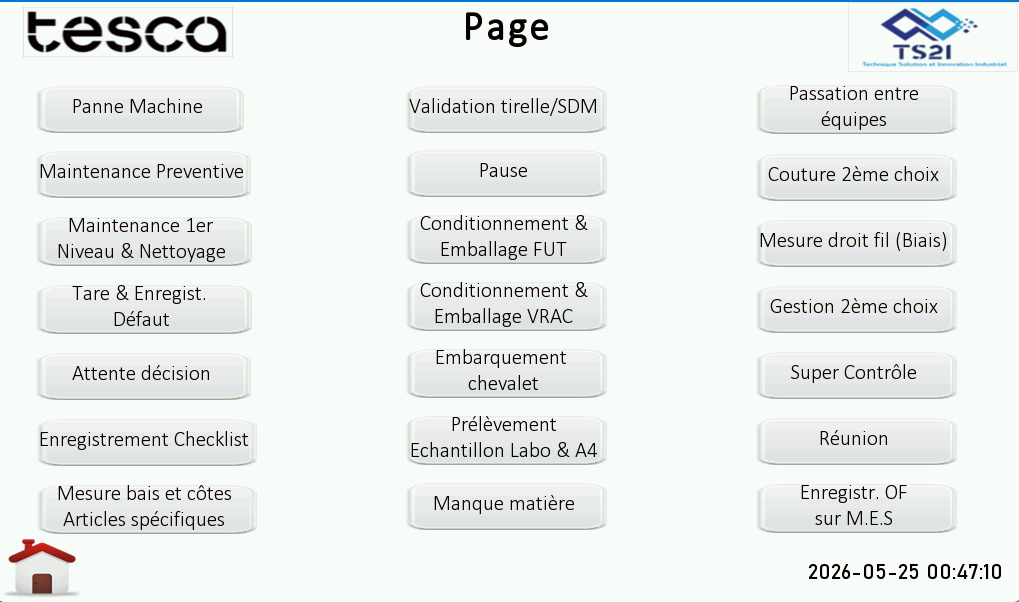
\includegraphics[width=0.75\textwidth, keepaspectratio]{images/hmi_veichi_vi20_cause_selection.png}
\caption{Veichi VI20 Local HMI - Stop-Cause Selection Screen}
\label{fig:chapter4-9}
\end{figure}

\subsection{Centralized Web HMI}
The web HMI was developed as a browser-based dashboard. It is served by the Node.js server and communicates with same-origin REST APIs. The Node.js server forwards validated commands to Node-RED, and Node-RED writes the corresponding Modbus coils or reads the required Modbus registers from the PLC.

The web HMI allows the user to send stop requests, follow restart authorization, display available causes and supervise the machine from the internal network. Safety-related functions remain handled by the PLC, the local safety devices and the existing machine safety chain.

\begin{figure}[H]
\centering
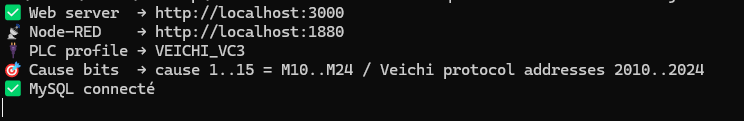
\includegraphics[width=0.5\textwidth, keepaspectratio]{images/web_hmi_runtime_status.png}
\caption{Runtime Status of the Web HMI Server and Communication Services}
\label{fig:chapter4-10}
\end{figure}

\begin{figure}[H]
\centering
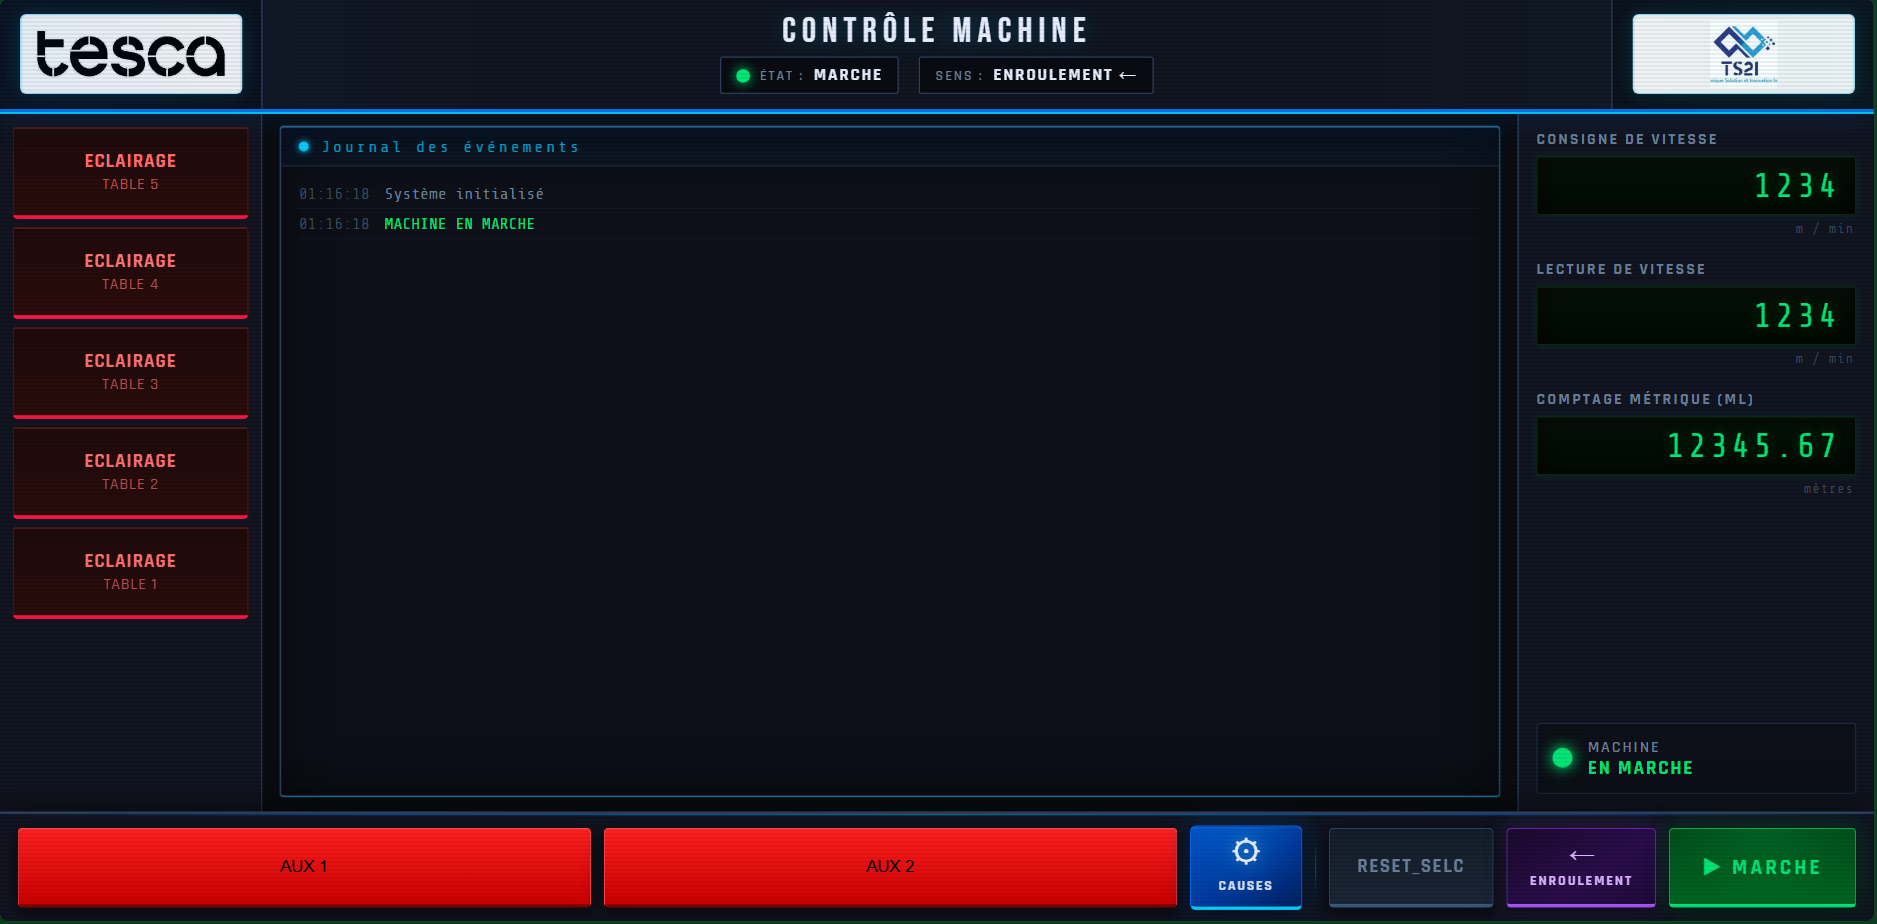
\includegraphics[width=0.85\textwidth, keepaspectratio]{images/hmi_web_dashboard_visiteuse2.png}
\caption{Web HMI - Supervision Dashboard}
\label{fig:chapter4-11}
\end{figure}

\begin{figure}[H]
\centering
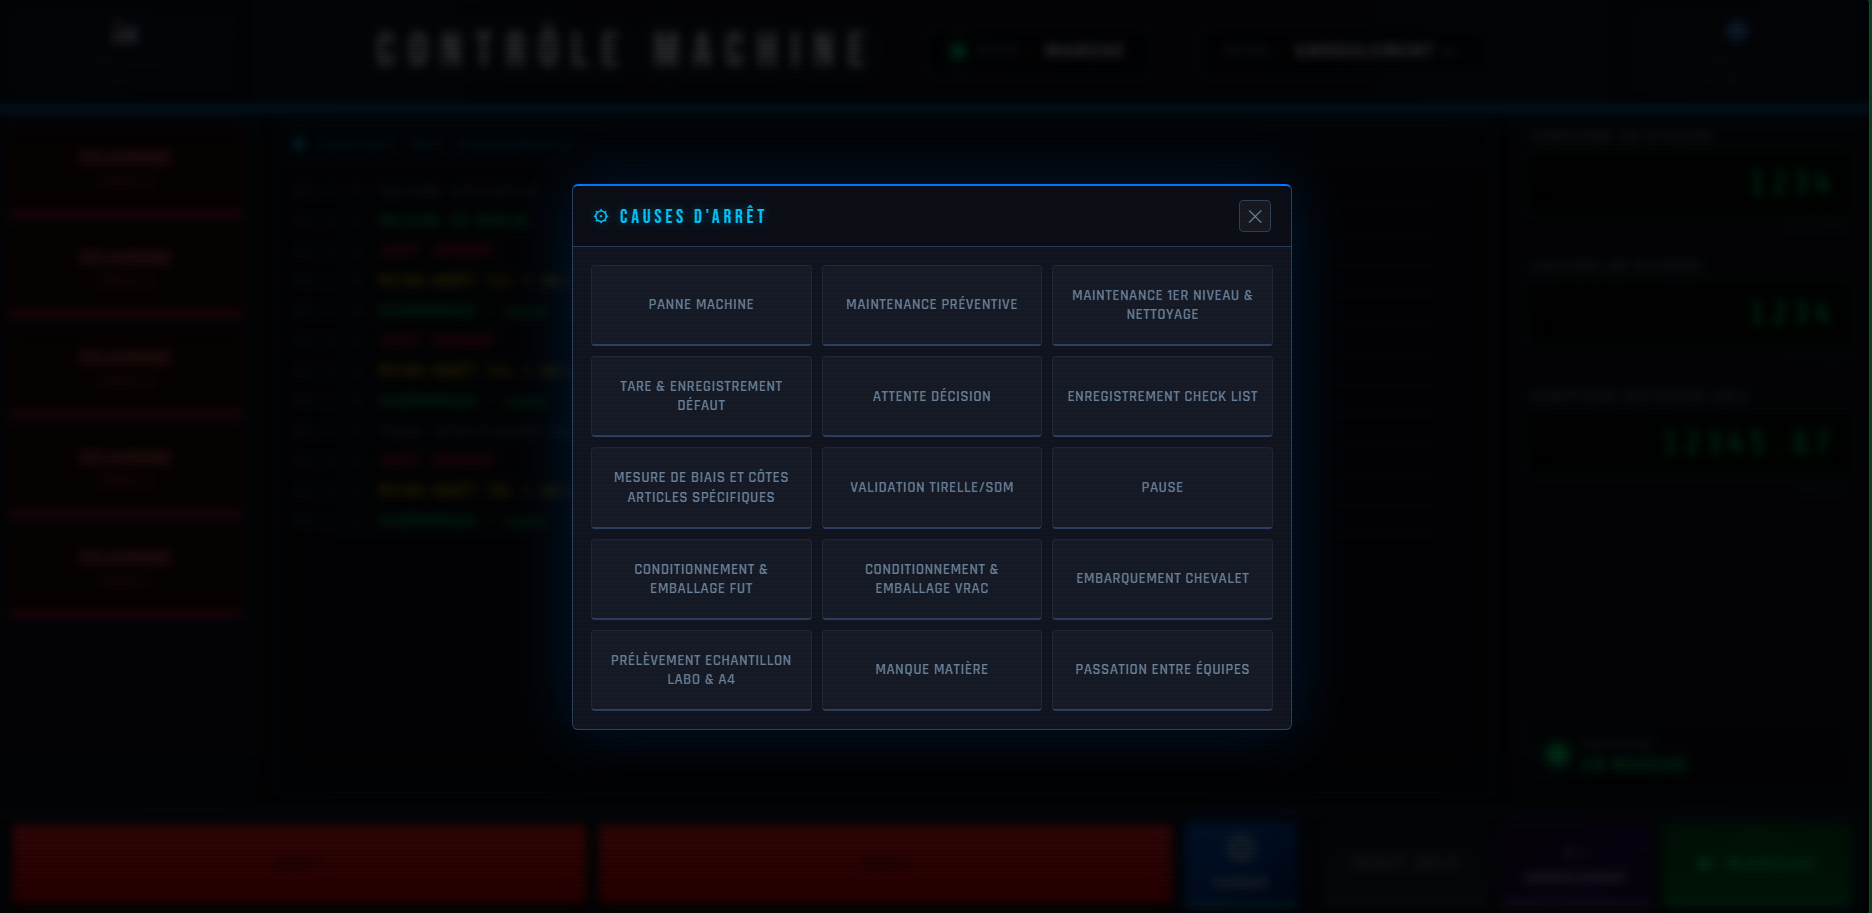
\includegraphics[width=0.85\textwidth, keepaspectratio]{images/hmi_web_stop_cause_selection.png}
\caption{Web HMI - Stop-Cause Selection Window}
\label{fig:chapter4-12}
\end{figure}

\begin{table}[H]
\centering
\caption{Main REST endpoints used by the web HMI}
\resizebox{\textwidth}{!}{%
\begin{tabular}{|l|l|p{6cm}|}
\hline
\textbf{Endpoint} & \textbf{Method} & \textbf{Function} \\
\hline
\texttt{/status} & \texttt{GET} & Returns the current web HMI state. \\
\hline
\texttt{/causes} & \texttt{GET} & Reads active causes from MySQL while excluding automatic cause \texttt{16}. \\
\hline
\texttt{/start-stop} & \texttt{POST} & Starts a stop cycle by writing \texttt{M0 = 1} through Node-RED. \\
\hline
\texttt{/end-stop} & \texttt{POST} & Sends the selected cause when required and closes the stop by resetting \texttt{M0}. \\
\hline
\texttt{/set-sens} & \texttt{POST} & Updates the selected winding direction; switching to \texttt{DEROULEMENT} triggers a stop cycle in the current implementation. \\
\hline
\end{tabular}%
}
\end{table}

\subsection{Complementarity Between the Local HMI and the Web HMI}
The local HMI and the web HMI serve different operational needs. The VI20 screen is used close to the machine for shop-floor operation, while the web interface provides remote supervision from an internal workstation.

\begin{table}[H]
\centering
\caption{Complementary roles of the two HMI layers}
\resizebox{\textwidth}{!}{%
\begin{tabular}{|l|l|l|}
\hline
\textbf{Criterion} & \textbf{VI20 local HMI} & \textbf{Web HMI} \\
\hline
Location & Installed near the machine. & Opened from an internal-network workstation. \\
\hline
Main user & Shop-floor operator. & Operator or production monitoring user. \\
\hline
Main role & Local operation and cause selection. & Centralized supervision and non-safety commands. \\
\hline
Communication path & Direct interaction with PLC variables. & Browser, Node.js server, Node-RED and PLC. \\
\hline
\end{tabular}%
}
\end{table}

\begin{figure}[H]
\centering
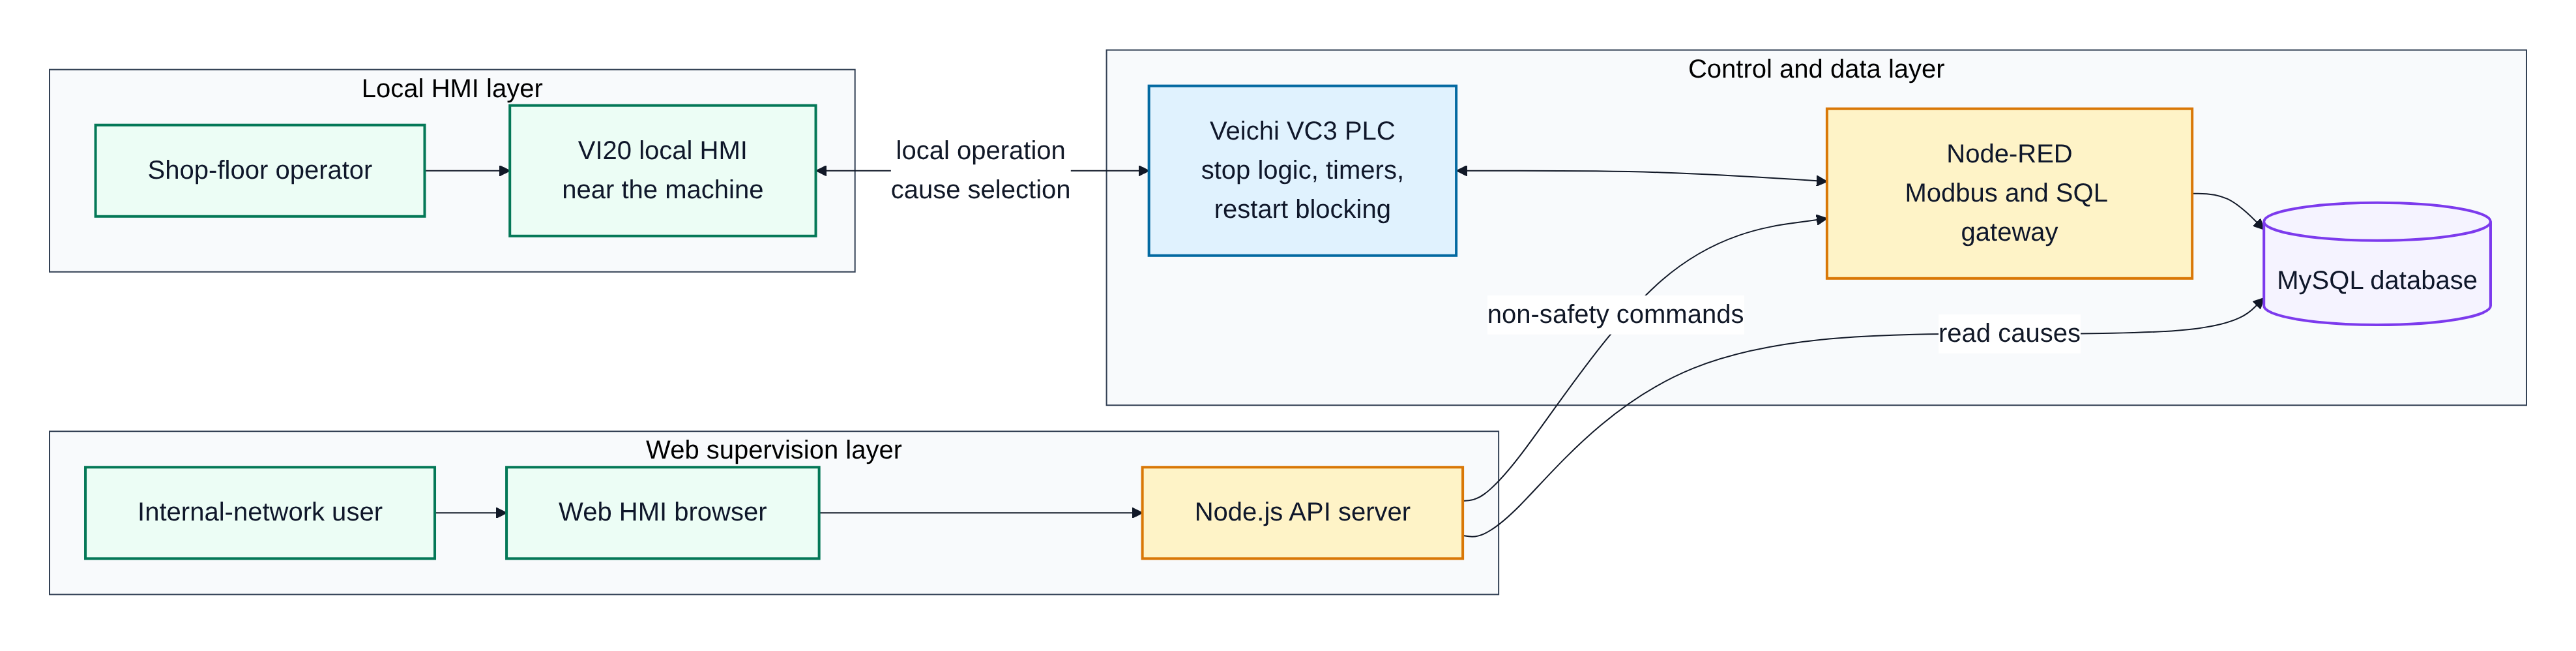
\includegraphics[width=0.9\textwidth, keepaspectratio]{images/fig_07_hmi_complementarity.png}
\caption{Complementary Roles of the Local HMI and the Web HMI}
\label{fig:chapter4-13}
\end{figure}

\section{Functional Validation of the Extension}

\subsection{Test Scenarios}
The extension was validated through the main operating scenarios of Visiteuse 2. The objective was to verify the consistency between the ladder logic, Modbus communication, HMI interaction and SQL recording. The main validation scenarios included short stops, long stops with cause selection, restart blocking, Modbus communication, web HMI operation and local HMI operation.

\subsection{Results Obtained}
The extension made it possible to deploy the stop-supervision principle on a second machine equipped with a different PLC platform. The ladder program was adapted to AutoStudio, the timers were implemented with TON blocks, the Modbus TCP profile was configured for the Veichi VC3 and the SQL insertion path was preserved.

The result confirms the feasibility of adapting the supervision method to Visiteuse 2. The implementation also provides a clear technical base for future reuse of the same principle, provided that each new machine receives its own PLC mapping and communication profile.

\section{Contribution of the Extension to the Project}

\subsection{Technical Contribution}
From a technical perspective, this extension made it possible to work on a new PLC platform and verify the portability of the stop-supervision principle. The transition to the Veichi VC3 PLC required timer adaptation, timestamp-register verification and precise configuration of Modbus addresses.

It also helped structure the system into clear layers: PLC logic, Node-RED communication, SQL recording, Node.js web API and HMI interaction.

\subsection{Industrial Contribution}
For the company, the main interest is the possibility of progressively reusing the same supervision principle on other machines. Visiteuse 2 serves as a concrete implementation example showing how the method can be adapted to another PLC while keeping a common operating logic.

The addition of the web HMI also improves usage flexibility. The operator keeps a local interface near the machine, while production users can access a centralized view from the internal network.

\subsection{Personal and Pedagogical Contribution}
On a personal level, this extension made it possible to go beyond a single-machine implementation. It provided experience with several technical environments and with the integration constraints between industrial automation, communication, database recording and web interfaces.

This experience strengthens the project because it demonstrates the ability to adapt an existing solution to a new industrial context.

\section*{Conclusion}
\addcontentsline{toc}{section}{Conclusion}
The extension to Visiteuse 2 shows that the stop-supervision principle can be adapted to a second production machine equipped with a Veichi VC3 PLC. The final solution combines ladder logic, Modbus TCP communication, Node-RED processing, SQL recording and two complementary HMI layers.
